\begin{figure}[]%H
\centering
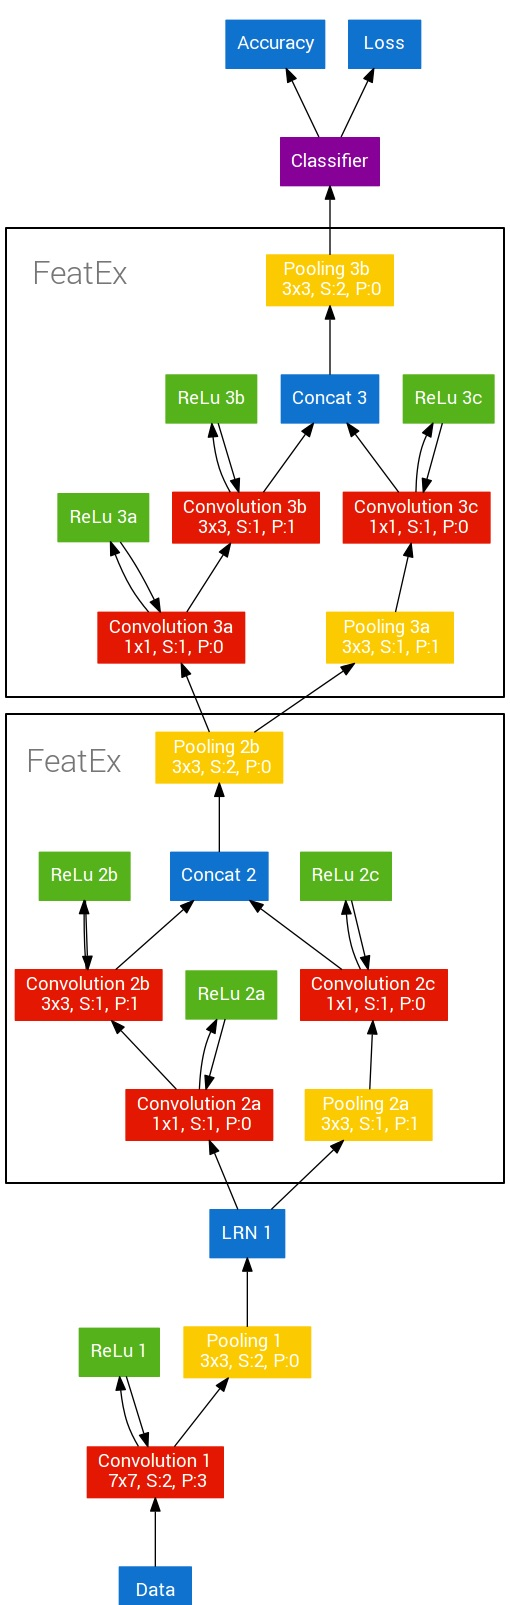
\includegraphics[scale=0.30]{Fig4}

\caption{This is the proposed architecture. The main component of this architecture is the FeatEx block. In the Convolutional layer $S$ depicts the Stride and $P$ the Padding.}
\label{fig:architecture}
\end{figure}


\section{Proposed Architecture}
\label{sec:architecture}


The proposed deep Convolutional Neural Network architecture (depicted in Figure~\ref{fig:architecture}) consists of four parts. The first part automatically preprocesses the data. This begins with Convolution 1, which applies $64$ different filters. The next layer is Pooling 1, which down-samples the images and then they are normalized by LRN 1. The next steps are the two FeatEx (Parallel Feature Extraction Block) blocks, highlighted in Figure~\ref{fig:architecture}. They are the core of the proposed architecture and described later in this section. The features extracted by theses blocks are forwarded to a fully connected layer, which uses them to classify the input into the different emotions.\\
The described architecture is compact, which makes it not only fast to train, but also suitable for real-time applications. This is also important as the network was built with resource usage in mind.

\begin{table}[ht!]
\centering
\caption{This Table lists the different output sizes produced by each layer.}
\label{tab:layers}

\begin{tabular}{l|l}
\hline
Layer & Output Size \\
\hline
Data & $224 \times 224$\\
Convolution 1 & $64 \times 112 \times 112$\\
Pooling 1 & $64 \times 56 \times 56$ \\
LRN 1 & $64 \times 56 \times 56$\\
\hline

Convolution 2a & $96 \times 56 \times 56$\\
Convolution 2b & $208 \times 56 \times 56$\\
Pooling 2a & $64 \times 56 \times 56$\\
Convolution 2c & $64 \times 56 \times 56$\\
Concat 2 & $272 \times 56 \times 56$\\
Pooling 2b & $272 \times 28 \times 28$\\
\hline

Convolution 3a & $96 \times 28 \times 28$\\
Convolution 3b & $208 \times 28 \times 28$\\
Pooling 3a & $272 \times 28 \times 28$\\
Convolution 3c & $64 \times 28 \times 28$\\
Concat 3 & $272 \times 28 \times 28$\\
Pooling 3b & $282 \times 14 \times 14$\\
\hline

Classifier & $11 \times 1 \times 1$\\
\hline
\end{tabular}
\end{table}

\paraV
\paragraph{\textit{FeatEx}}
The key structure in our architecture is the Parallel Feature Extraction Block (FeatEx). It is inspired by the success of GoogleNet. The block consists of Convolutional, Pooling, and ReLU Layers. The first Convolutional layer in FeatEx reduces the dimension since it convolves with a filter of size $1\times1$. It is enhanced by a ReLU layer, which creates the desired sparseness. The output is then convolved with a filter of size $3\times3$. In the parallel path a Max Pooling layer is used to reduce information before applying a CNN of size $1\times1$. This application of differently sized filters reflects the various scales at which faces can appear.\\
The paths are concatenated for a more diverse representation of the input. Using this block twice yields good results.\\


\paraV
\paragraph{\textit{Visualization}}
The different layers of the architecture produce feature vectors as can be seen in Fig~\ref{fig:feature_extraction}.
The first part until LRN 1 preprocesses the data and creates multiple modified instances of the input. These show mostly edges with a low level of abstraction. The first FeatEx block creates two parallel paths of features with different scales, which are combined in Concat 2. The second FeatEx block refines the representation of the features. It also decreases the dimensionality.\\
This visualization shows that the concatenation of FeatEx blocks is a valid approach to create an abstract feature representation. The output dimensionality of each layer can be seen in Table \ref{tab:layers}.

\begin{figure}[ht]
\centering
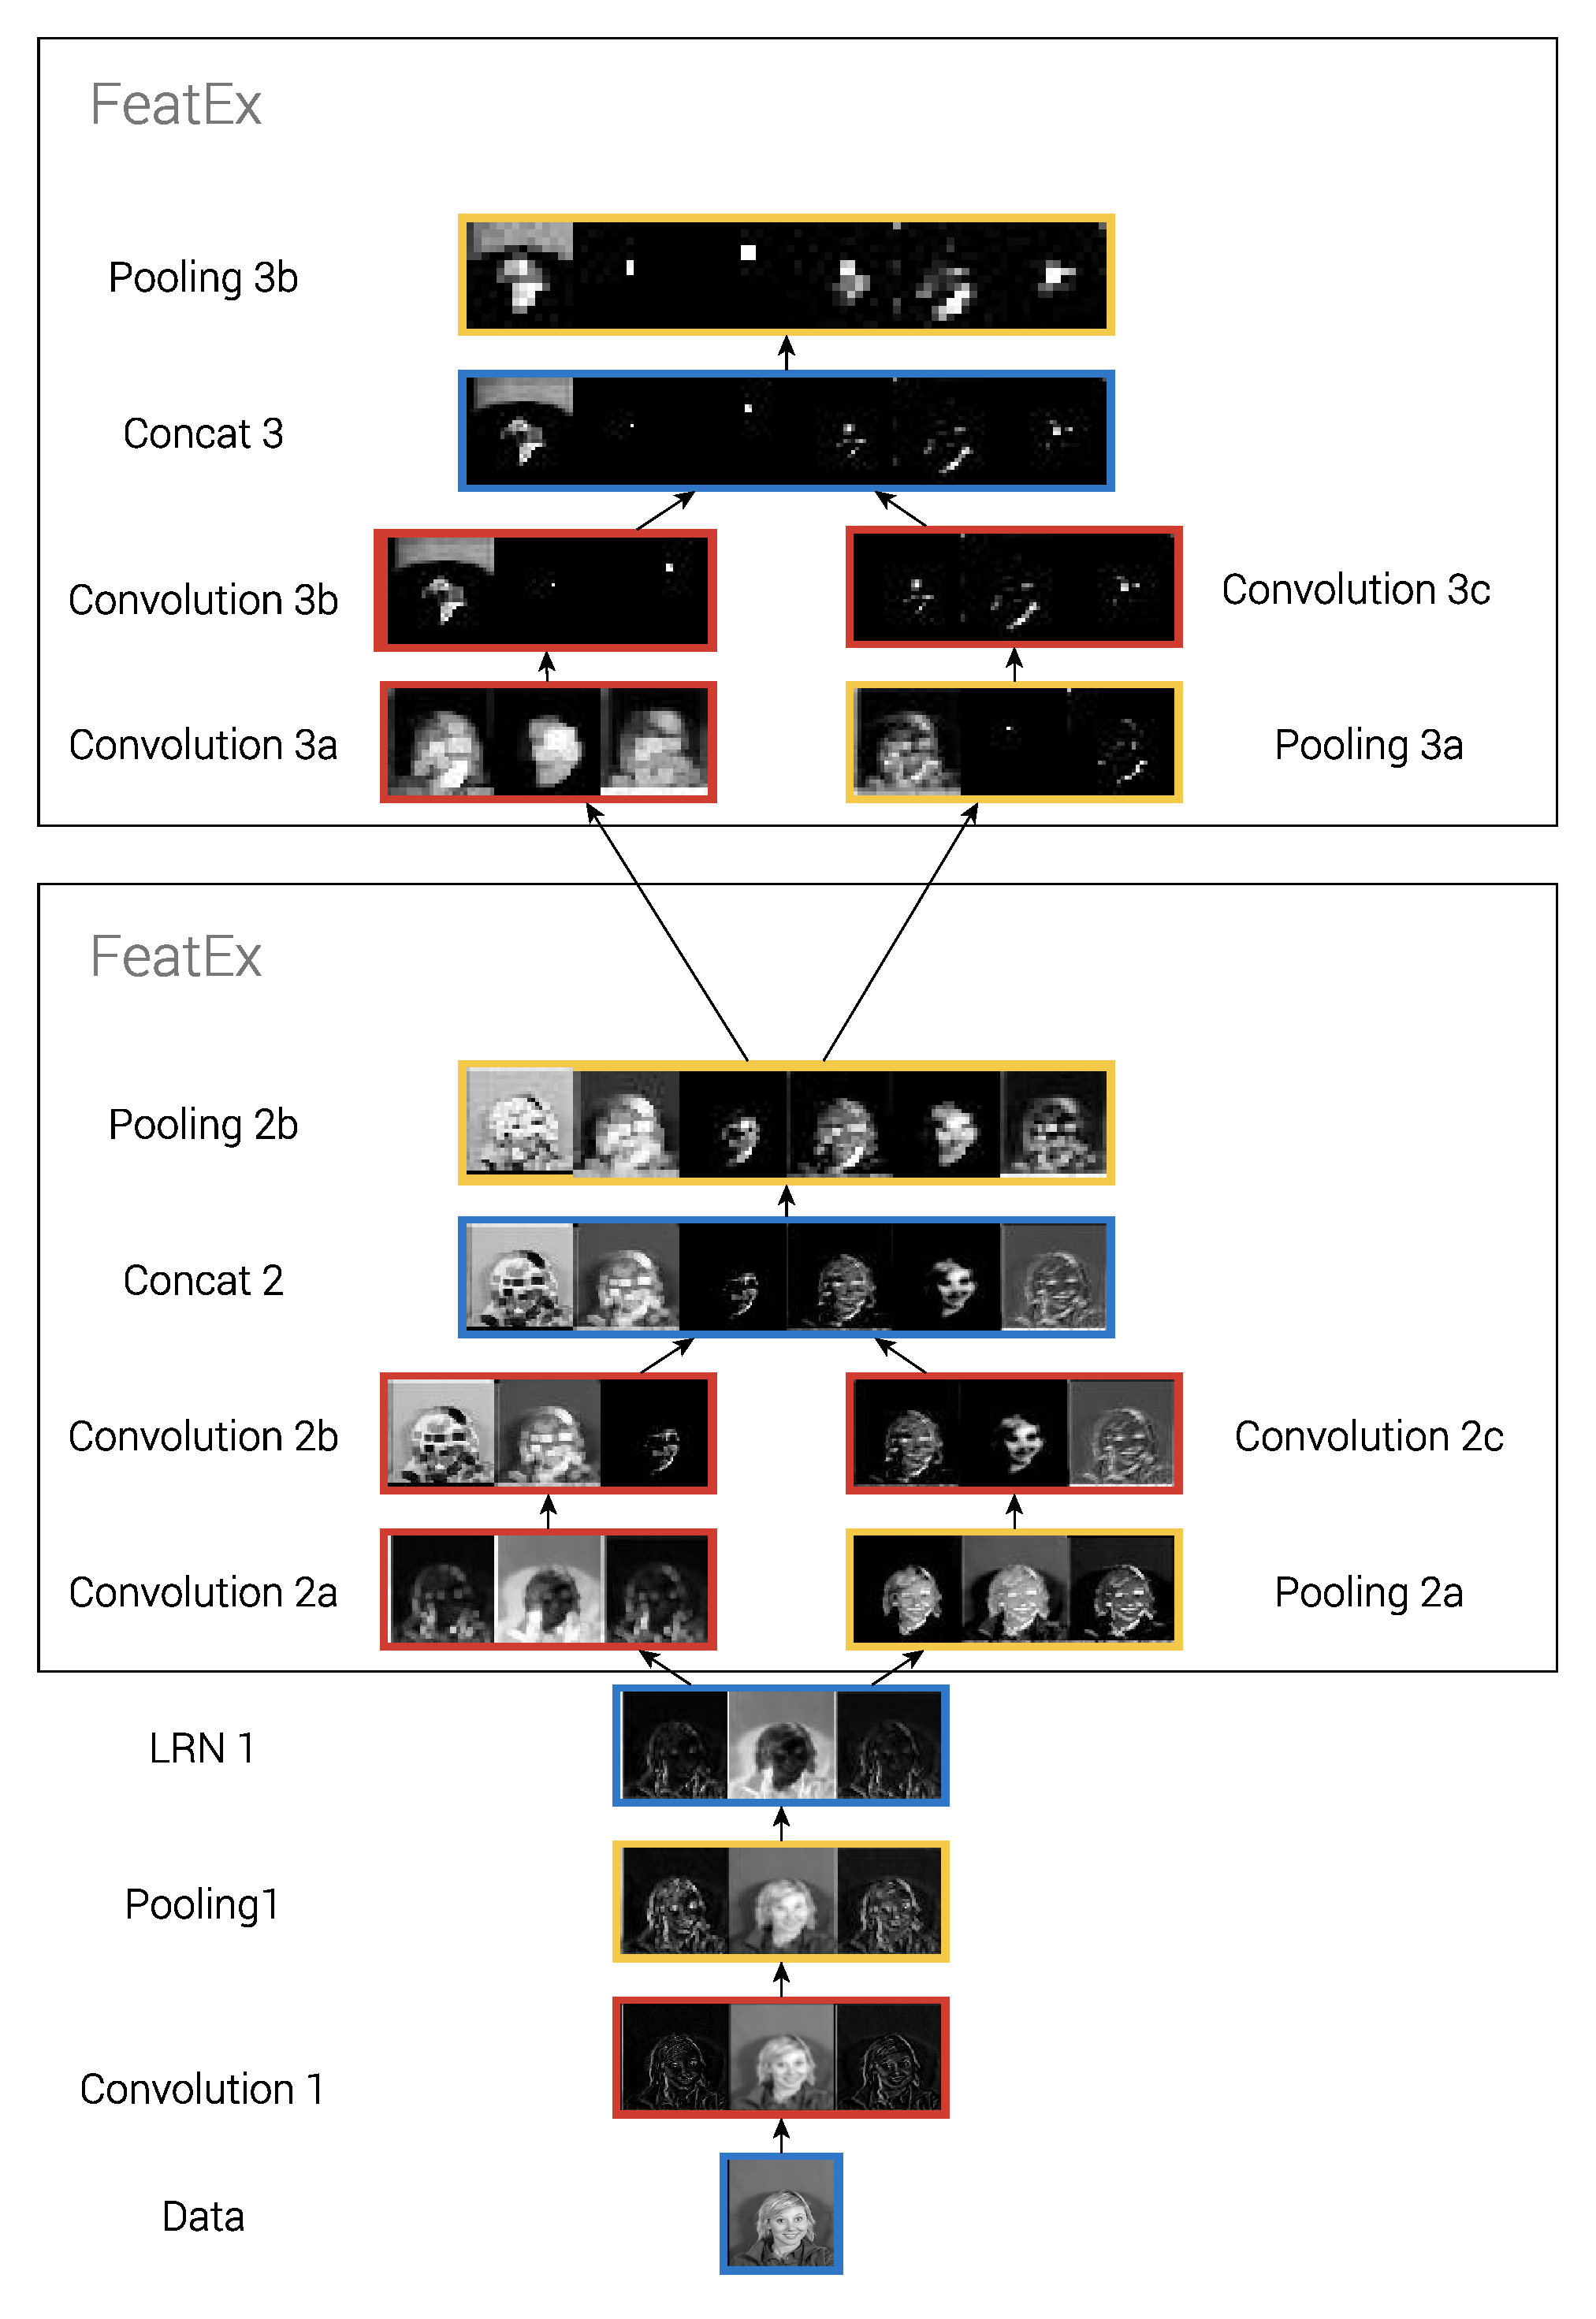
\includegraphics[width=\columnwidth]{Fig5.eps}
\caption{This Figure shows example visualizations of the different layers. The data is taken from the MMI set.}
\label{fig:feature_extraction}
\end{figure}